\section{Darboux Integral}

\subsection{Rectangles and Partitions}
\begin{definition}[Rectangle]
A rectangle $R \subseteq \R^n$ is a set defined by
$$
R = [a_1,b_1] \times [a_2, b_2] \times \cdots \times [a_n, b_n]
$$
for some $a_1<b_1,\;\cdots a_n < b_n$.
\end{definition}

\begin{definition}[Partition of Interval]
Given a closed interval $[a,b]$ of $\R$, a partition of $[a,b]$ is a finite collection $P \subseteq [a,b]$ of points of $[a,b]$ that includes the points $a$ and $b$.
$$
a = t_0 < t_1 < \cdots < t_k = b
$$
\end{definition}

\begin{definition}[Partition of Rectangle]
Given a rectangle $R = [a_1,b_1] \times [a_2, b_2] \times \cdots \times [a_n, b_n]$, the partition of $R$ is an $n$-tuple $P=(P_1,\cdots,P_n)$ where $P_i$ is a partition of $[a_i,b_i]$. Intuitively, we break the rectangle $R$ into finitely many subrectangles.

If $P_i$ contains $k_i$ many subintervals, then the partition $P$ of $R$ contains $\prod_{i=1}^n k_i$ many subrectangles.
\end{definition}

\subsection{Refinement}

\begin{definition}[Refinement]
If $P$ and $Q$ are two partitions of a rectangle $R$. We say that $Q$ is a refinement of $P$ if
$$
\forall i,\; Q \subset P'
$$
\end{definition}

\begin{lemma}[Common Refinement]
Given two partitions $P$ and $Q$, one can always find a partition $O = P \cup Q$ that is finer than both $P$ and $Q$.
\end{lemma}

\begin{lemma}
If $Q$ is a refinement of $P$, then
$$
L_Q f \geq L_P f \qquad U_Q f \leq U_Q f
$$
\end{lemma}

\begin{lemma}
For every two partitions $P$ and $Q$,
$$
L_P f \leq U_Q f
$$
\end{lemma}

All these three lemmas were proven when we were first introduced to Darboux integral for single-variable functions.

\subsection{Darboux Sums}
\begin{definition}[Lower and Upper Darboux Sum]
Let $R$ be a rectangle in $\R^n$; let $f:\; R \to \R$. Assume $f$ is bounded. Let $P$ be a partition of $R$. For each subrectangle $S$ determined by $P$, let
$$
\begin{aligned}
m_S(f) &= \inf\{f(\vv x) \mid \vv x \in S\} \\
M_S(f) &= \sup\{f(\vv x) \mid \vv x \in S\}
\end{aligned}
$$
We define the lower and upper Darboux sum, respectively, of $f$, determined by $P$, as
$$
\begin{aligned}
L_P f &= \sum_S m_S(f) \cdot v(S) \\
U_P f &= \sum_S M_r(f) \cdot v(S)
\end{aligned}
$$
\end{definition}

\subsection{Integral}

\begin{definition}[Lower and Upper Integrals]
Let $R$ be a rectangle. Let $f:\; R \to \R$ be a bounded function. We define the Darboux lower and upper integral, respectively, as
$$
\underline{\int_R}f = \sup \{ L_P f \mid \text{$P$ is a partition of $R$ }\} \qquad
\overline{\int_R}f = \inf \{ U_P f \mid \text{$P$ is a partition of $R$ }\}
$$
\end{definition}

\begin{center}
    \begin{tikzpicture}
    \draw[>=triangle 45, <->] (-4,0) -- (4,0);
    \draw (-1,0.2) -- ++ (0,-0.4) node[font=\large, below] {$\underline{\int_R}f$};
    \draw (1,0.2) -- ++ (0,-0.4) node[font=\large, below] {$\overline{\int_R}f$};
    \foreach \x in {0.5,1,1.5,...,10} {
        \draw (-1 - 1 / \x,0) node[circle,fill,inner sep=1.5pt,color=red] {};
    }
    \foreach \x in {0.5,1,1.5,...,10} {
        \draw (1 + 1 / \x,0) node[circle,fill,inner sep=1.5pt,color=codegreen] {};
    }
    \end{tikzpicture}
\end{center}

\begin{definition}[Integral]
Let $R$ be a rectangle. Let $f:\; R \to \R$ be a bounded function. If $\underline{\int_R}f = \overline{\int_R}f$, we say that $f$ is Darboux integrable over $R$. And we define the integral to be their common value
$$
\int_R f = \underline{\int_R}f = \overline{\int_R}f
$$
\end{definition}


\subsection{Remarks}

\begin{theorem}[$\varepsilon$ criterion for integrability]
Let $R$ be a rectangle. Let $f:\; R \to \R$ be a bounded function.
$$
\text{$f$ is integrable over $R$} \iff \forall \varepsilon > 0,\; \exists \text{ partition $P$},\; U_P f - L_P f < \varepsilon
$$
\end{theorem}


\section{Double Integral Over Rectangles}

\subsection{Definition}

\begin{definition}[Double integral as a double Riemann sum]
The double integral of $f$ over the rectangle $R$ is
$$
\iint_R f(x,y) dA = \lim_{m,n \to \infty} \sum_{i=1}^m \sum_{j=1}^n f(x_{ij}^*, y_{ij}^*) \Delta A
$$
if the limit exists. We say the function $f$ is integrable if this limit exists.
\end{definition}

\subsection{Geometric Meaning}
If $f(x,y) \geq 0$, then the volume $V$ of the solid that lies above the rectangle $R$ and below the surface $z=f(x,y)$ is
$$
V = \iint_R f(x,y) dA
$$

\begin{figure}[h]
    \centering
    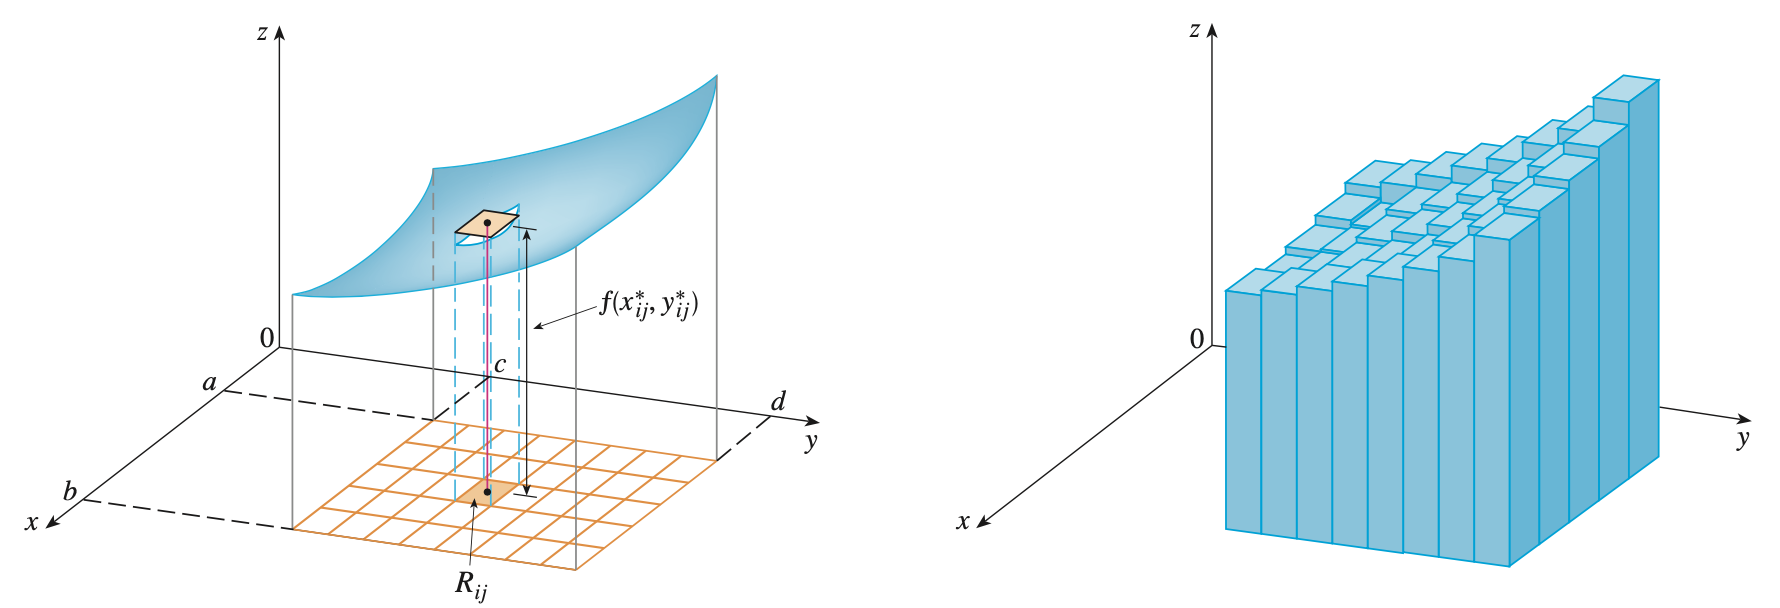
\includegraphics[width=0.6\linewidth]{figures/double-Riemann.png}
    \caption{The volume under the surface}
    \label{fig:geometric_doubleInt}
\end{figure}

\subsection{Iterated Integral}

We can evaluate a double integral over a rectangle using a method known as iterated integrals. Suppose we have a Riemann integrable function $f:\; \R^2 \to \R$ and we want to integrate it over the rectangle $R=[a,b]\times[c,d]$. We first calculate the area of the slice by integrating it with respect to $y$. This is called the partial integral with respect to $y$.
$$
A(x) = \int_c^d f(x,y) dy
$$
Then, to get the volume, we integrate $A(x)$ with respect to $x$.
$$
V = \int_a^b A(x) dx = \int_a^b\int_c^d f(x,y) dy dx
$$

Similar to the Clairaut's Theorem for mixed partial derivative, there is a theorem stating that interated integral is also symmetric.

\begin{theorem}[Fubini's Theorem]
If $f$ is continuous on the rectangle $R = \{(x,y) \mid a \leq x \leq b,\, c \leq y \leq b$ \}, then
$$
\iint_R f(x,y) dA = \int_a^b \int_c^d f(x,y) dy dx = \int_c^d \int_a^b f(x,y) dx dy
$$
\end{theorem}

\section{Double Integral Over Non-rectangles}
\subsection{Defining the Region of Integration}

It is a little bit trickier to compute a double integral over a general region. Instead of using constants when defining limits of integration, the limit of integration for one variable may be a function of the other variable.

Generally, there are two types of non-rectangular regions
$$
D = \left\{(x,y)\in \R^2 : a\le x \le b, \phi(x) \le y \le \psi(x)\right\}
$$
\begin{figure}[h]
    \centering
    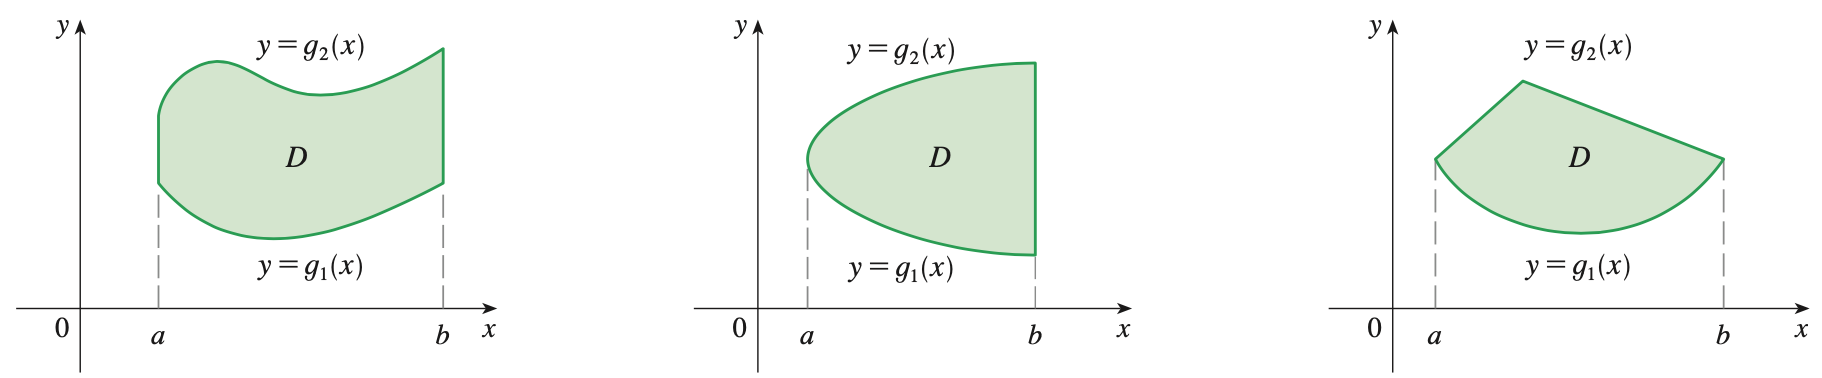
\includegraphics[width=\linewidth]{figures/type1-gen-region.png}
\end{figure}

and

$$
D = \left\{(x,y)\in \R^2 : c\le y \le d, \phi(y) \le x \le \psi(y)\right\}
$$
\begin{figure}[h]
    \centering
    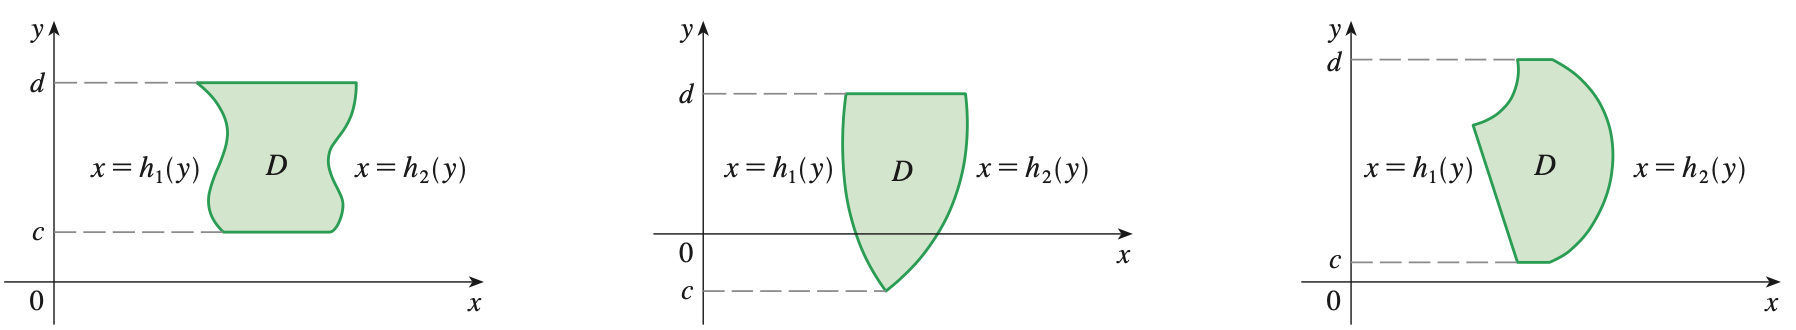
\includegraphics[width=\linewidth]{figures/type2-gen-region.png}
\end{figure}

Then, the double integral over such regions can be written as either
$$
\iint_D f\, dA =  \int_a^b \left( \int_{\phi(x)}^{\psi(x)} f(x,y) dy\right)dx
$$
or
$$
\iint_D f\, dA =  \int_a^b  \left( \int_{\phi(y)}^{\psi(y)}  f(x,y) dx\right)dy
$$

\subsection{Changing the Order of Integration}

Fubini's Theorem allows us to swap the order of integration when evaluating double integrals.

\begin{example}
Swap the order of integration for $\int_0^1 \int_x^1 \sin(y^2)dy\, dx$.

From the limits of integration, we know the region of integration is
$$
D = \{ (x,y) \mid 0 \leq x \leq 1,\, x \leq y \leq 1 \}
$$
which can also be equivalently expressed as
$$
D = \{ (x,y) \mid 0 \leq y \leq 1,\, 0 \leq x \leq y \}
$$
Hence, the integral can be rewrite as
$$
\int_0^1 \int_0^y \sin(y^2) dx\, dy
$$
\end{example}

\subsection{Combining Regions of Integration}
If $D = D_1 \cup D_2$ where $D_1$ and $D_2$ do not overlap except maybe on their boundaries, then
$$
\iint_D f(x,y) dA = \iint_{D_1} f(x,y) dA + \iint_{D_2} f(x,y) dA
$$
Using this properties, we can integrate over regions that are neither Type I or II.
\begin{figure}[h]
    \centering
    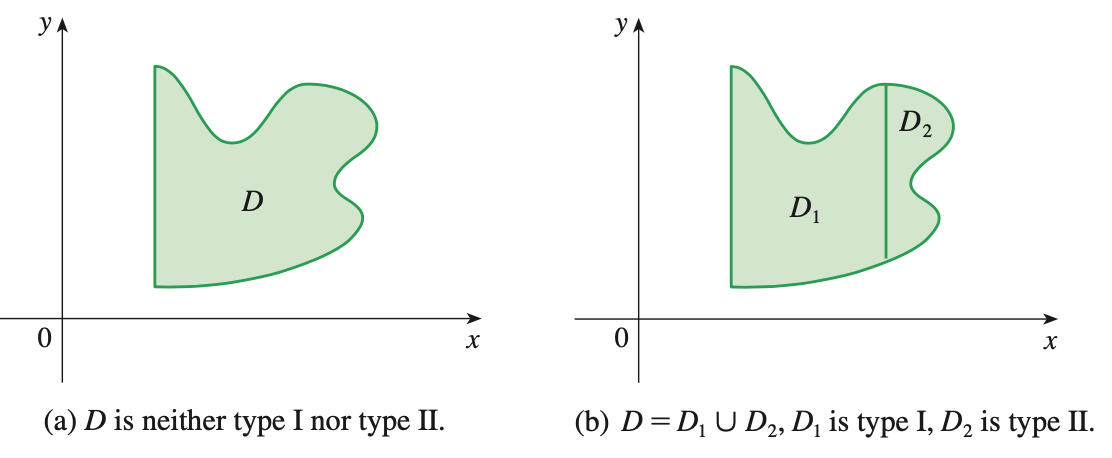
\includegraphics[width=0.7\linewidth]{figures/combine-region.png}
    \caption{Combining regions of integration}
    \label{fig:combine_regions}
\end{figure}

\section{Change of Variable}

\begin{theorem}[Change of Variable Theorem]
$$
\int_T f(\vv u) d\vv u = \int_{\vv G^{-1}(T)} f(\vv G(x)) |\det D\vv G(\vv x)|\, d\vv x
$$
\end{theorem}

\section{Double Integral in Polar Coordinates}

\section{Applications of Double Integral}